\section[Advice]{General advice}

\subsection{}

\begin{frame}
    \frametitle{Hardware}
    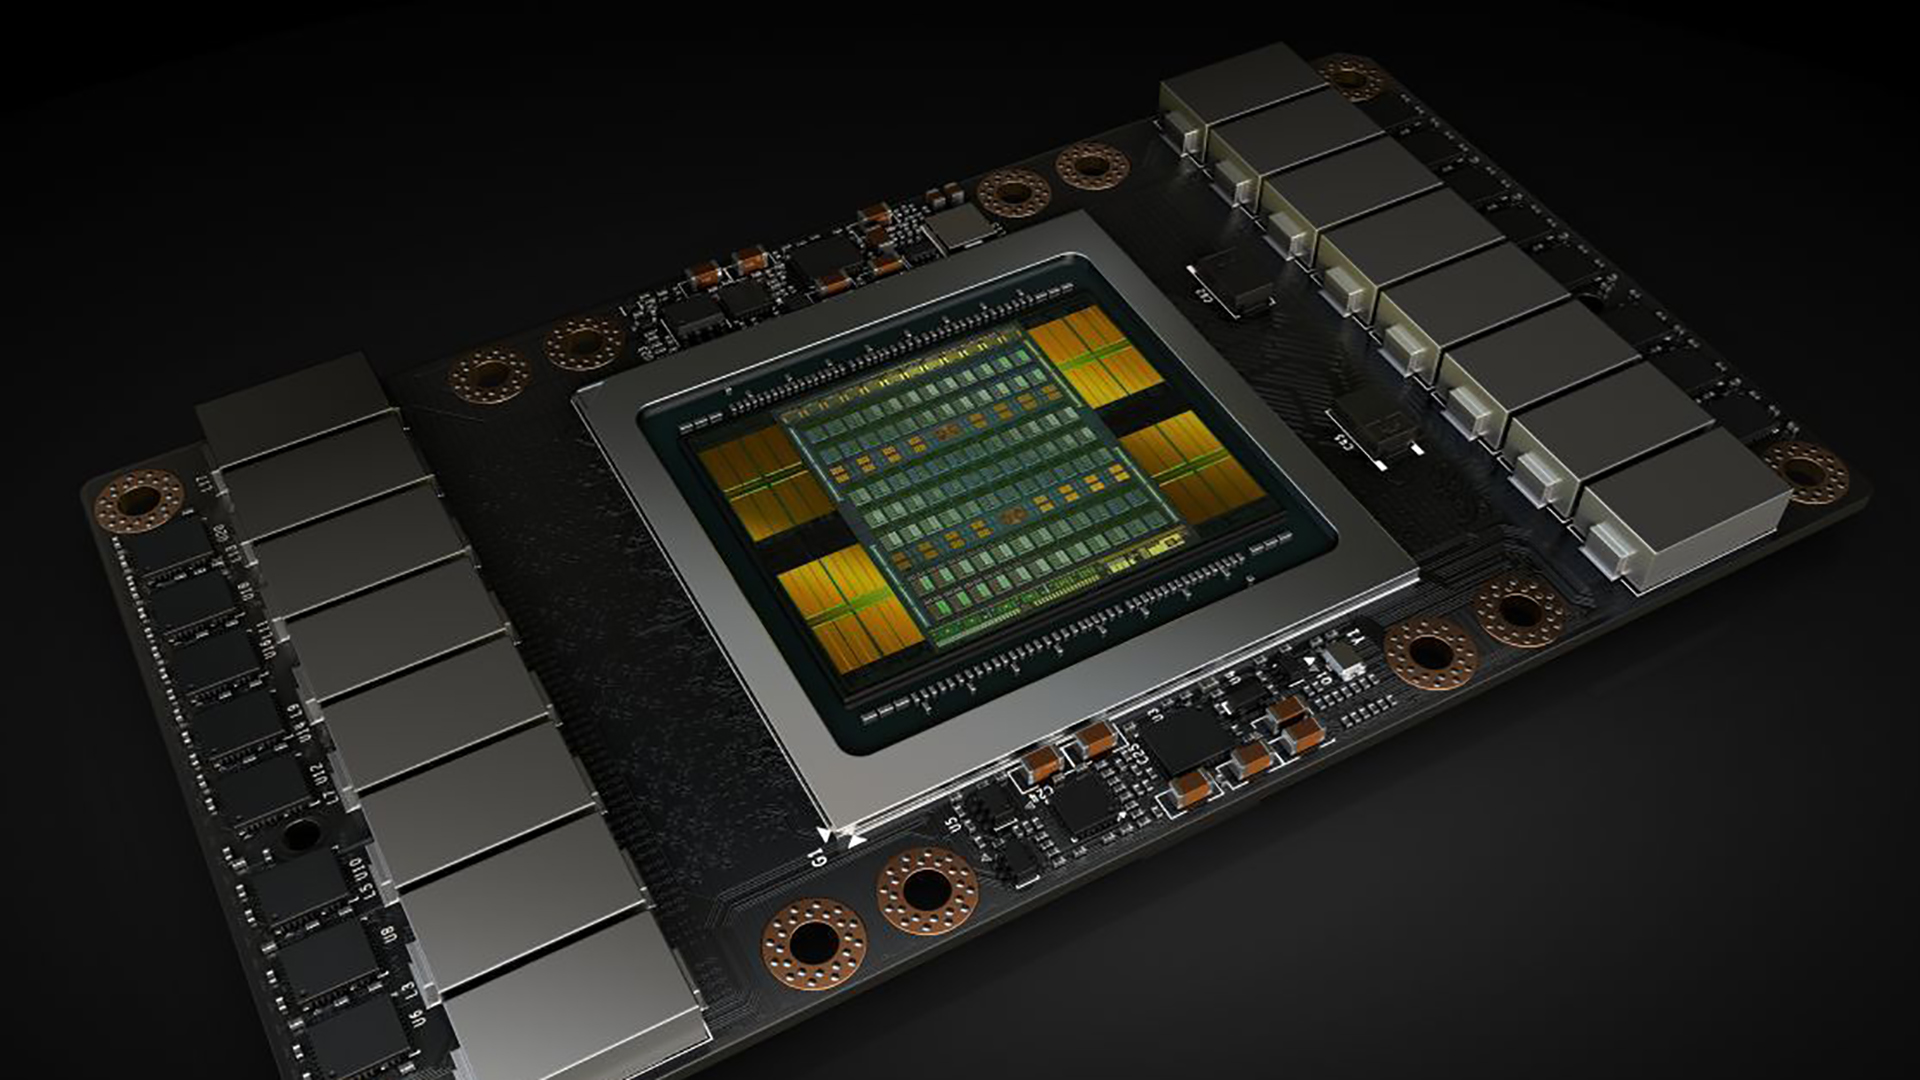
\includegraphics[width=0.48\textwidth]{volta}
    \hfill
    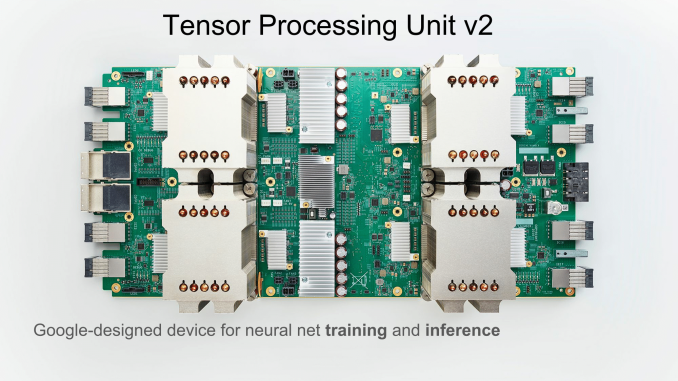
\includegraphics[width=0.48\textwidth]{tpu}

    \begin{itemize}[<+->]
        \item \alert{Use GPUs.}
        The bulk of forward and backprop is matrix--vector multiplies; common for GPUs to be $\O(10 \text{--} 100)\times$ faster than CPUs
        \item \alert{Use GPUs built for NNs.}
        NVIDIA Volta and Google tensor processing unit (TPU) are built from ground-up to be lightning fast for NNs (e.g., 16-bit multiply-add for 32-bit result)
        \item \alert{Use mini-batch sizes and widths that are integer powers of 2.}
        Not a hard rule, but GPUs tend to more efficient this way
        \item \alert{Use 32-bit floats.}
        Neural networks are not turbulence simulations; no tangible benefit to 64-bit doubles
    \end{itemize}
\end{frame}

\begin{frame}
    \frametitle{Software}
    \begin{itemize}
        \item $\exists$ many NN platforms; unclear which will win out in the end.
        \item Most popular now: Keras, TensorFlow, PyTorch
        \begin{itemize}
            \item TensorFlow seems to be winning, but list changes rapidly
        \end{itemize}
        \pause
        \item How do they compare in my opinion?
    \end{itemize}

    \begin{center}
        \begin{tikzpicture}
    \def\pos{0}
    \scale{difficult}{easy}
    \entry{TF}{-3}
    \entry{PT}{-1}
    \entry{K}{3}

    \def\pos{-1.5}
    \scale{limited \\ capability}{flexible}
    \entry{K}{-3}
    \entry{TF}{1.7}
    \entry{PT}{3}

    \def\pos{-3}
    \scale{limited \\ docs}{excellent \\ docs}
    \entry{K}{-1.2}
    \entry{TF}{1.5}
    \entry{PT}{3}

    \def\pos{-4.5}
    \scale{small \\ user base}{large \\ user base}
    \entry{PT}{-1.5}
    \entry{K}{1}
    \entry{TF}{3}
\end{tikzpicture}
%%% Local Variables:
%%% mode: latex
%%% TeX-master: "../nn"
%%% End:

    \end{center}
\end{frame}

\begin{frame}
    \frametitle{Neural network architecture}
    \begin{tikzpicture}[node distance=3mm]
    \dropoutnetwork{green}

    \foreach \i/\j in {
        0/1, 0/3, 0/4, 1/0, 1/1, 1/2, 1/4, 2/0, 2/1, 2/2, 2/3, 2/4%
    } {
        \draw (input \i) -- (dense 0\j);
    }

    \foreach \i/\j in {
        0/0, 0/1, 0/2, 1/0, 1/1, 1/2, 1/3, 2/2, 3/0, 3/2, 4/0, 4/1, 4/2%
    } {
        \draw (dense 0\i) -- (dense 1\j);
    }

    \foreach \i/\j in {
        0/0, 1/0, 1/1, 2/1, 3/1%
    } {
        \draw (dense 1\i) -- (output \j);
    }
\end{tikzpicture}
%%% Local Variables:
%%% mode: latex
%%% TeX-master: "../nn"
%%% End:

    \hfill
    \begin{tikzpicture}[node distance=3mm]
    \dropoutnetwork{green}

    \foreach \i/\j in {
        0/1, 0/2, 0/3, 0/4, 1/0, 1/1, 1/2, 1/3, 2/0, 2/1, 2/2, 2/4%
    } {
        \draw (input \i) -- (dense 0\j);
    }

    \foreach \i/\j in {
        0/2, 1/1, 1/2, 1/3, 2/0, 2/1, 2/3, 3/0, 3/1, 4/0, 4/1%
    } {
        \draw (dense 0\i) -- (dense 1\j);
    }

    \foreach \i/\j in {
        1/0, 2/0, 2/1%
    } {
        \draw (dense 1\i) -- (output \j);
    }
\end{tikzpicture}
%%% Local Variables:
%%% mode: latex
%%% TeX-master: "../nn"
%%% End:

    \hfill
    \begin{tikzpicture}[node distance=3mm]
    % Box.
    \draw [fill=green!10, rounded corners] (-0.75, -0.25) rectangle (1.75, 1.75);

    % Nodes.
    \node (input 0) [io mini] {};
    \node (input 1) [io mini, right=of input 0] {};
    \node (input 2) [io mini off, right=of input 1] {};

    \node (dense 01) [neuron mini off, above=of input 0] {};
    \node (dense 00) [neuron mini off, left=of dense 01] {};
    \node (dense 02) [neuron mini, right=of dense 01] {};
    \node (dense 03) [neuron mini off, right=of dense 02] {};
    \node (dense 04) [neuron mini, right=of dense 03] {};

    \node (dense 10) [neuron mini off, above=of dense 00, xshift=2.5mm] {};
    \node (dense 11) [neuron mini, right=of dense 10] {};
    \node (dense 12) [neuron mini, right=of dense 11] {};
    \node (dense 13) [neuron mini, right=of dense 12] {};

    \foreach \i in {0, 1} {
        \pgfmathtruncatemacro{\j}{\i + 1}
        \node (output \i) [io mini, above=of dense 1\j] {};
    }

    % Connections.
    \foreach \i in {2, 4} {
        \foreach \j in {0, 1} {
            \draw (input \j) -- (dense 0\i);
        }

        \foreach \j in {1, ..., 3} {
            \draw (dense 0\i) -- (dense 1\j);
        }
    }

    \foreach \i in {1, ..., 3} {
        \foreach \j in {0, 1} {
            \draw (dense 1\i) -- (output \j);
        }
    }
\end{tikzpicture}
%%% Local Variables:
%%% mode: latex
%%% TeX-master: "../nn"
%%% End:

    \hfill
    \begin{tikzpicture}[node distance=3mm]
    % Box.
    \draw [fill=blue!10, rounded corners] (-0.75, -0.25) rectangle (1.75, 1.75);

    % Nodes.
    \node (input 0) [io mini] {};

    \foreach \i in {1, 2} {
        \pgfmathtruncatemacro{\j}{\i - 1}
        \node (input \i) [io mini, right=of input \j] {};
    }

    \foreach \i in {0, ..., 2} {
        \pgfmathtruncatemacro{\j}{\i + 1}
        \node (dense 0\j) [neuron mini, above=of input \i] {};
    }

    \node (dense 00) [neuron mini, left=of dense 01] {};
    \node (dense 04) [neuron mini, right=of dense 03] {};

    \foreach \i in {0, ..., 3} {
        \node (dense 1\i) [neuron mini, above=of dense 0\i, xshift=2.5mm] {};
    }

    \foreach \i in {0, 1} {
        \pgfmathtruncatemacro{\j}{\i + 1}
        \node (output \i) [io mini, above=of dense 1\j] {};
    }

    % Connections.
    \foreach \i in {0, ..., 4} {
        \foreach \j in {0, ..., 2} {
            \draw (input \j) -- (dense 0\i);
        }

        \foreach \j in {0, ..., 3} {
            \draw (dense 0\i) -- (dense 1\j);
        }
    }

    \foreach \i in {0, 1} {
        \foreach \j in {0, ..., 3} {
            \draw (dense 1\j) -- (output \i);
        }
    }
\end{tikzpicture}
%%% Local Variables:
%%% mode: latex
%%% TeX-master: "../nn"
%%% End:


    \begin{itemize}[<+->]
        \item \alert{Start with architectures that are too small.}
        NNs take a long time to train; make problems show up immediately.
        \item \alert{Scale up architectures until they overfit.}
        Check the relation between NN size and validation loss.
        Back off on size if validation loss increases.
        \item \alert{Use dropout.}
        They are one of the best regularizers.
        \item \alert{Aim for $\text{\# parameters} \le \text{\# data}$.}
        Helps prevent overfitting.
        \item \alert{Let layer $i$ be \sfrac{1}{2}--\sfrac{3}{4} the width of layer $i - 1$.}
        Layers closer to the input have greater expressive power.
        \item \alert{Beware of excessive depth.}
        They make NNs much harder to train.
    \end{itemize}
\end{frame}

\begin{frame}
    \frametitle{End-to-end machine learning}
\end{frame}

\begin{frame}
    \frametitle{Data}

    \begin{itemize}
        \item<+-> \alert{Normalize the data, or use batch normalization.}
        NNs learn better if inputs look standard normal and uncorrelated.
        \item<+-> \alert{Be wary of extrapolation.}
        Statistical models are meaningless outside their domain of training.
        \begin{itemize}
            \item E.g., sigmoid/ReLU activations have 0th/1st order extrapolation
        \end{itemize}
    \end{itemize}

    \begin{columns}
        \begin{column}{0.4\textwidth}
            \centering
            \footnotesize

            \uncover<+->{
                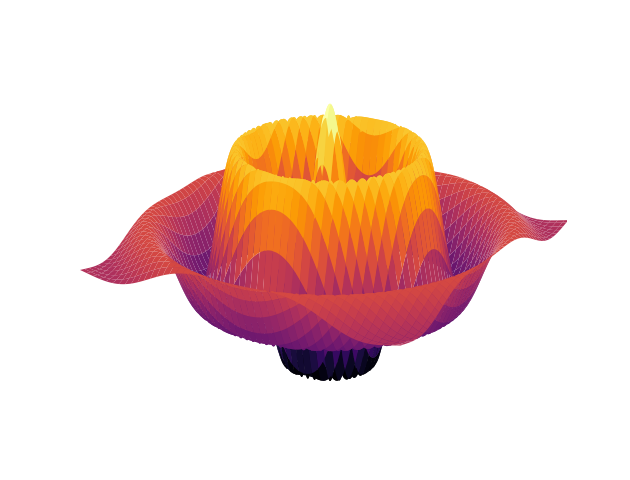
\includegraphics[width=1.5in]{ripple} \\
                ground truth, $[-12, 12] \times [-12, 12]$
                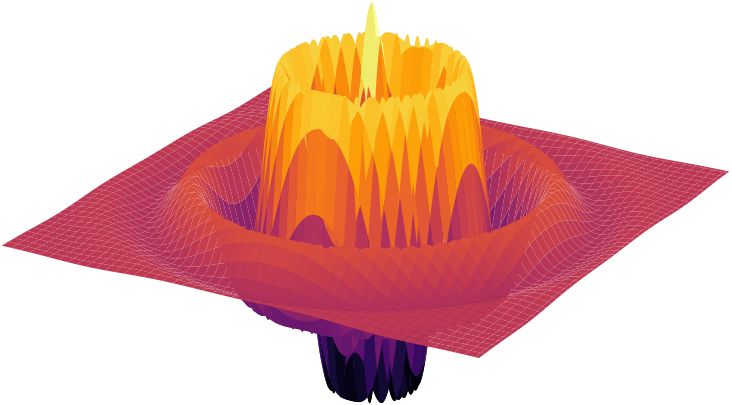
\includegraphics[width=1.5in]{extended_ripple} \\
                ground truth, $[-18, 18] \times [-18, 18]$
            }
        \end{column}

        \begin{column}{0.6\textwidth}
            \centering
            \footnotesize

            \uncover<+->{
                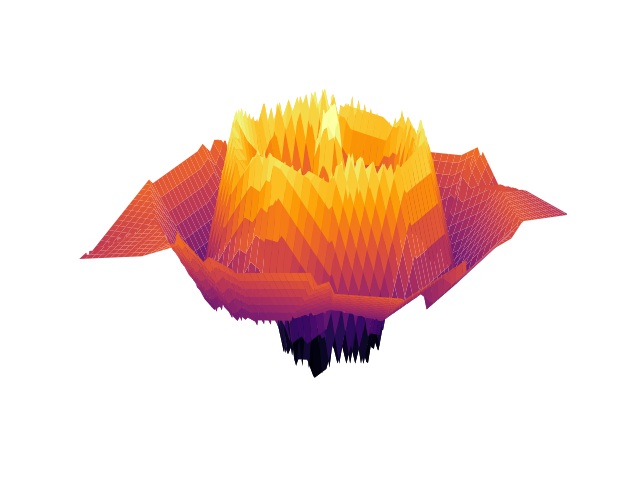
\includegraphics[width=1.5in]{ripple_2layer} \\
                17--8 neurons, $[-12, 12] \times [-12, 12]$
                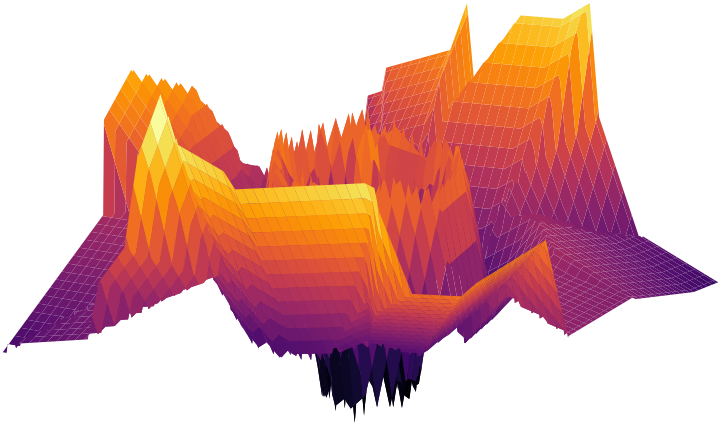
\includegraphics[width=1.5in]{extrapolated_ripple} \\
                above model extrapolated to $[-18, 18] \times [-18, 18]$
            }
        \end{column}
    \end{columns}
\end{frame}

\begin{frame}
    \frametitle{Engaging with the scientific community}
    % Obsolete papers.
    % Interpretability criticisms
\end{frame}

%%% Local Variables:
%%% mode: latex
%%% TeX-master: "../nn"
%%% End:
